\section{Materials and Methods}\label{sec:materials-and-methods}

\subsection{Motivating Datasets}\label{sec:motivating-datasets}

A \emph{data object} refers to the type and structure of the basic ``atom" of a statistical analysis (i.e., a single observation) \parencite[][p.1]{marron_object_2021}.
In univariate statistics, the object is a number (i.e., scalar), and in classical multivariate statistics, observations comprise $p$ variables and are represented as $p$-dimensional vectors.
In recent years, as highlighted by \textcite[Chapter 1]{marron_object_2021}, there has been an emergence of techniques for the analysis of more general and complex data objects such as smooth time-varying curves \parencite{ramsay_functional_2005}, spiky signals \parencite{morris_wavelet-based_2006}, images \parencite{morris_automated_2011}, shapes \parencite{srivastava_shape_2011}, trees \parencite{wang_object_2007}, probability distributions \parencite{petersen_functional_2016} and correlation/ covariance matrices \parencite{desai_connectivity_2023}.
In most cases, a suitable transformation of the observed object data to a (typically lower-dimensional and Euclidean) space of latent features facilitates the application of familiar statistical approaches to the complex objects.

In principle, GLaRe can be applied to any type of complex object dataset whose observations can be stored in a vector, matrix or array. 
In this section, we introduce three motivating object datasets that can be viewed as functional data defined on two-dimensional Euclidean or spherical domains.

\subsubsection{Glaucoma Data}

Glaucoma is considered a leading factor in blindness. It is characterized by damage to the optic nerve related by which can be measured through \emph{intraocular pressure (IOP)}. 
To investigate proposed hypotheses about the relationship between glaucoma and IOP, \textcite{fazio_age-related_2014} developed instrumentation to measure the mechanical strain on the scleral surface of the eye at different levels of IOP. 
The measurements were summarized for each location at different locations on the scleral surface of the eye as \emph{maximum principal strain} (MPS). MPS was computed on 34 eyes from 19 normal human donors. It was measured in the posterior globe of both eyes on a partial spherical domain with $120$ circumferential locations $\upsilon \in (0^{\circ}, 360^{\circ})$ and $120$ meridional locations $\theta \in (9^{\circ}, 24^{\circ})$.
These measurements were taken at 9 different IOP levels. 
One study goal for this dataset was to test the hypothesis that scleral strain decreases with age thereby causing damage to the optic nerve head which could lead to glaucoma \parencite{lee_bayesian_2019}.
Figure \ref{fig:combined-data-objects} (a) displays is a two-dimensional polar azimuthal projection of a single observation from the Glaucoma data.

We let $X_i(t)$ denote the MPS function for a single eye at a specific IOP level so that $i = 1, \dots, N = 306$ ($34$ eyes at $9$ IOP levels).
The data lives on a domain $\mathcal{T}$ which is the portion of the sphere defined by $(\upsilon, \theta)$ for $\upsilon \in (0^{\circ}, 360^{\circ})$ and $\theta \in (9^{\circ}, 24^{\circ})$.
Therefore, each observation $X_i(t)$ is recorded a common grid of size $T = 14400$.
The recordings are indexed by the $14400$-dimensional vector $\mathbf{t} = \boldsymbol{\upsilon} \times \boldsymbol{\theta}$, where $\boldsymbol{\upsilon}$ represents $120$ equally-spaced measurements of $\upsilon$ along $(0^{\circ}, 360^{\circ})$ and $\boldsymbol{\theta}$ represents $120$ equally-spaced measurements of $\theta$ along $(9^{\circ}, 24^{\circ})$.
We denote the vector of measurements for the $i$th observation as $X_i(\mathbf{t})$, so that the full datsaset can be represented by the $N \times T$ data matrix $\mathbf{X}$, containing $X_1(\mathbf{t}), \dots, X_N(\mathbf{t})$ in its rows.

\subsubsection{Proteomic Gels Data}

In neurobiology, a particularly important issue is the identification of changes responsible for the transition from non-dependent drug use to addiction which is characterized by drug intake behavior. Studies done on rats have shown that rats given a 6-12 hours/day access of cocaine or heroin have significant increase in drug intake while rats given 1 hour/day access kept the same level of intake overtime.
The corresponding neurochemical changes in the extended part of the brain amygdala relate to cellular effects that affect protein expression and function which can be detected via proteomic analysis. To study this phenomenon, experiments were done on rats in which the rats were trained to get cocaine by pressing a lever: 6 rats were given 1hour/day access, 7 rats were given 6 hours /day access and 8 rats were used for control with no access to the cocaine. The rats were euthanized after some time, and their brains studied \parencite{morris_pinnacle_2008}. 
Two-dimensional gel electrophoresis was used to study the proteomic content in the brain tissues. 
Between two and three gels were obtained from each rat and brain region, resulting in a dataset of 53 gel images from 21 rats.
Each gel image has $556,206$ pixel intensities observed on a $646 \times 861$ grid. 
A research goal for this dataset was to study the proteins which are differentially expressed in brains of rats that were exposed to cocaine for a long time versus those that were not.
This can be done by finding regions in the gel images where image intensity is significantly different across groups \parencite{morris_statistical_2012}. 
Figure \ref{fig:combined-data-objects} (b) displays a single gel image observation.

We denote a single observation from the proteomic gels dataset as $X_i(t)$, where $i=1, \dots, N = 53$.
Here, $t$ represents a location $(t_1, t_2)$ in the two-dimensional Euclidean domain defined by the Cartesian product $\mathcal{T} = [0, 1] \times [0, 1]$.
Measurements of each observation are made at the vector of locations $\mathbf{t} = \mathbf{t}_1 \times \mathbf{t}_2$ where $\mathbf{t}_1$ and $\mathbf{t}_2$ represent vectors of $646$ and $861$ equally-spaced points along $[0, 1]$, respectively.
Then $X_i (\mathbf{t})$ denotes the $T = 556206 ( = 646 \times 861)$-dimensional vector containing the measurements of the $i$th observation at the locations in $\mathbf{t}$, and the $N \times T$ data matrix $\mathbf{X}$ contains $X_1 (\mathbf{t}), \dots, X_N (\mathbf{t})$ in its rows.


\subsubsection{MNIST Digits Data}

The MNIST (Modified National Institute of Standards and Technology) database of handwritten digits was compiled by \textcite{lecun_mnist_1998}, from a larger collection of images from the National Institute of Standards and Technology (NIST).
It comprises a training set of $60000$ images and a test set of $10000$ images, representing hand-written digits from $0$ to $9$ (i.e., $10$ distinct digits/ classes).
The original black and white images from NIST were modified into $28 \times 28$ pixel greyscale images.
The MNIST dataset has been employed extensively in computer vision and deep learning applications as a test case for image reconstruction and digit identification/ classification models.
The dataset can be represented in an $N \times T$ matrix $\mathbf{X}$ where $N = 60000$ (in the case of the training set) and $T= 784 (= 28 \times 28)$.
We let $X_i(t)$ represent the value of the $i$th greyscale image at pixel location $t$, where $t \in \mathbf{t} = \{1, \dots, 28\} \times \{1, \dots, 28\}$.
Then the $i$th row of the data matrix $\mathbf{X}$ contains the $784$-dimensional vector $X_i(\mathbf{t})$, i.e., measurements of the $i$th observation at the vector of pixel locations in $\mathbf{t}$.
We normalise the greyscale images so that $X_i(t) \in [0, 1]$ for all $t \in \mathbf{t}$ and $i = 1, \dots, N$. 
Figure \ref{fig:combined-data-objects} (c) displays a single digit from the MNIST dataset.
The full dataset (training and test) is publicly available in the \pkg{keras} \proglang{R} package \parencite{kalinowski_keras_2024} and can be loaded using the \texttt{dataset\_mnist()} function.





\begin{figure}
    \centering
    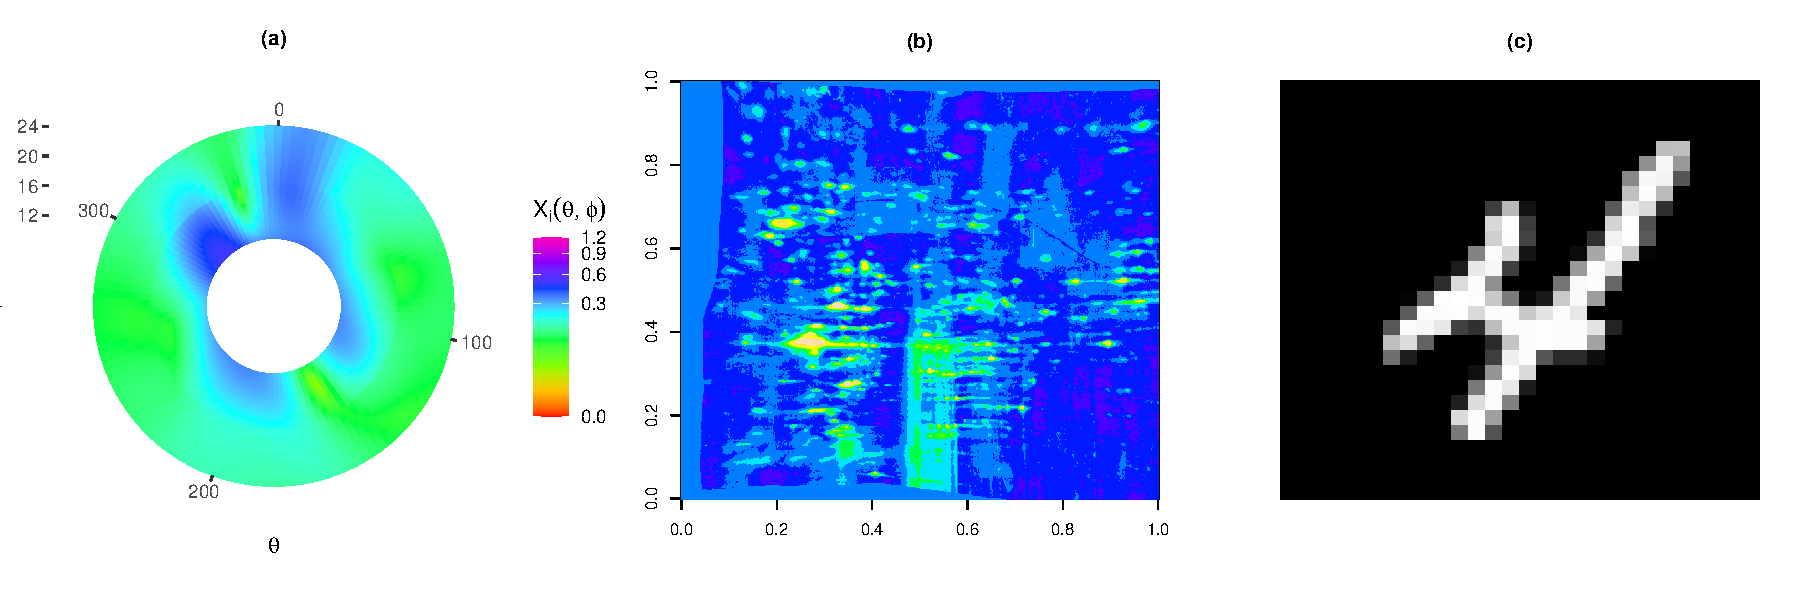
\includegraphics[width=1\textwidth]{figures/data-plot.pdf}
    \caption{
    A sample observation from each of our three motivating datasets.
    \textbf{(a)}: A sample glaucoma image, representing a polar azimuthal projection of MPS functions for a single eye at one IOP level.
    \textbf{(b)}: A sample 2D gel electrophoresis image, showing proteomic content in the brain tissue of a rat.
    \textbf{(c)}: A sample MNIST digit image, which is a $28 \times 28$ pixel greyscale image of single handwritten digit.}
    \label{fig:combined-data-objects}
\end{figure}

\subsection{Latent Feature Representations}

Suppose that we have $N$ observations of object data, denoted by $X_1 (t), \dots, X_N(t)$, where $t$ indexes a location on a domain $\mathcal{T}$ over which the objects are defined.
For time-varying curves, $\mathcal{T}$ is generally a closed subset of the real line that represents a (normalized) time interval.
However, as exemplified in our three motivating datasets, the domain $\mathcal{T}$ can be multi-dimensional to represent locations in an image or surface, and it can also be non-Euclidean ({see Glaucoma data/ \textcite{lee_bayesian_2019}}).
We assume that each observation is measured on a common\footnote{In practice, the measurement grids of individual observations need not be identical if they are all sufficiently fine such that interpolation onto a common, fine grid is feasible.}, ordered grid of $T$ points in $\mathcal{T}$, denoted by $\mathbf{t} = \left(t_1, \dots, t_T\right)^\top$, and we let $X_i(\mathbf{t}) = \left(X_i(t_1), \dots, X_i(t_T)\right)^\top$.
Then, we can represent the observed data in the $N \times T$ data matrix $\mathbf{X}$, which contains the vectors $X_1(\mathbf{t}), \dots, X_N(\mathbf{t})$ in its rows.
We refer to the $T$-dimensional space of features in which the observed data are represented as the \emph{data space}.

We define a \emph{latent feature representation method} as a technique comprising two transformations, known as the \emph{encoding} and \emph{decoding} transforms.
The encoding transform $f_{K}$ transforms an observation from the data space to a new space of latent features, called the \emph{representation space}
$$
f_{K} \left(X_i(\mathbf{t})\right) = \left(X_{i1}^*, \dots,  X_{iK}^* \right)^\top,
$$
where the number of features $K$ defines the dimensionality of the representation space and can range between $1$ and some possible maximum $K_{max}$. When $K \ll T$, we say that the latent feature representation is \emph{sparse}.
As we expand on in Section \ref{sec:characterising-information-loss}, we typically want the representation space to be as sparse as possible.

% space\footnote{If we have have representation of the underlying object $X_i(t)$ that does not involve measurement on a grid, the transformation can be defined on the object itself as $f_{K} \left(X_i(t)\right) = \left(X_{i1}^*, \dots,  X_{iK}^* \right)^\top$.} to a new space of latent features, called the \emph{representation space}, and back-transforms on observation in the latent space of features to the data space, using an inverse transformation.
% Mathematically, we define the latent feature representation of the $i$th observation as



We define the decoding transform as the inverse transformation function $f^{-1}_K$ that maps an observation from the representation space back to the data space as
$$
\widehat{X}_i(\mathbf{t}) = f_{K}^{-1} \left( \left(X_{i1}^*, \dots,  X_{iK}^* \right)^\top \right).
$$

Linear transformations of the form $f_{K} \left(X_i(\mathbf{t})\right) = \mathbf{A} X_i(\mathbf{t})$, for some $K \times T$ transformation matrix $\mathbf{A}$, are often used in practice.
For example, it is common to represent a functional observation $X_i(t)$ as a linear combination of a set of basis functions $\{\phi_k(t)\}_{k=1}^K$, which defines the inverse transformation
$$
\widehat{X}_i(\mathbf{t}) = \sum_{k=1}^K X_{ik}^* \phi_k(\mathbf{t}) = \boldsymbol{\Phi} \left(X_{i1}^*, \dots,  X_{iK}^* \right)^\top,
$$
where $\boldsymbol{\Phi} = \left[\phi_1(\mathbf{t}) | \dots | \phi_K(\mathbf{t}) \right]$ and the latent features $X_{ik}^*$ are basis coefficients. 
When these basis coefficients are computed by ordinary least squares, the linear transformation matrix defining the latent feature representation $f_K$ is of the form $\mathbf{A} = \left( \boldsymbol{\Phi}^\top \boldsymbol{\Phi} \right)^{-1} \boldsymbol{\Phi}^\top$.
When the matrix of basis function evaluations $\boldsymbol{\Phi}$ is orthogonal, $\mathbf{A} = \boldsymbol{\Phi}^\top$, i.e., the transformation $f_K$ is simply right multiplication by this matrix.
However, in general, there is no need for the transformation $f_K$ to be orthogonal or even linear, and non-linear transformations may be preferred for certain types of data.

\subsection{Assessing Losslessness via Generalization Error}

Although statistical modelling is performed in the representation space due to its attractive properties, we often want to transform modelling results back to the data space for inference, interpretation and visualisation. 
As such, the accuracy and interpretation of an analysis depends on the degree of information that is preserved when moving back and forth between the data and representation spaces for a given latent feature representation.
In what follows, we characterise the degree of information loss of a latent feature representation on a full dataset.


\subsection{Characterising Information Loss}\label{sec:characterising-information-loss}

We characterise the degree of information loss of a latent feature representation for each individual observation as
$$
\text{Loss} \left( f_K(X_i(t)) \right) = \lVert  X_i(\mathbf{t}) - f^{-1}_{K}(X_{ik}^*) \rVert,
$$
{\color{purple}where $\lVert \boldsymbol{\cdot} \rVert$ denotes a measure (e.g., $\mathcal{L}_2$ norm) such that $\lVert  X_i(\mathbf{t}) - f^{-1}_{K}(X_{ik}^*) \rVert$ defines a distance between $X_i(\mathbf{t})$ and $f^{-1}_{K}(X_{ik}^*)$ \parencite{morris_comparison_2017}}.
We say that the transformation $f_K$ is \emph{lossless} for the $i$th observation $X_i(t)$ if
$$
\text{Loss} \left( f_K(X_i(\mathbf{t})) \right) = 0,
$$
and lossless for the full dataset $X_1(t), \dots, X_N (t)$ if
$$
\text{Loss} \left( f_K(X_i(\mathbf{t})) \right) = 0 \quad \forall \quad  i = 1, \dots, N.
$$
That is, we only refer to a latent feature representation as lossless for a given dataset if the representation is near lossless for every individual observation in that dataset.
More generally, we can allow some tolerance of information loss and say that
the transformation $f_K$ is \emph{near-lossless} for the $i$th observation $X_i(t)$ if
$$
\text{Loss} \left( f_K(X_i(\mathbf{t})) \right) < \epsilon,
$$
for a chosen tolerance level $\epsilon$. 
Similarly, we say that the transformation $f_K$ is near-lossless for the full dataset only if each individual observation achieves this tolerance level, that is
$$
\text{Loss} \left( f_K(X_i(\mathbf{t})) \right) < \epsilon \quad \forall \quad  i = 1, \dots, N.
$$
In this case, it is important to note that the distinction between this definition and a measure such as the average of individual losses $\frac{1}{N}\sum_{i=1}^N \text{Loss} \left( f_K(X_i(\mathbf{t})) \right)$.
For example, Figure \ref{fig:ind-losses} displays the distribution of individual information losses on a dataset sample dataset of a PCA latent of varying dimensions.
In this case, we are using the squared correlation measure as our loss, so a value $0$ means the representation captures no information and a value of $1$ means that the representation is lossless.
The grey points represent the individual observations' losses, whereas the red squares indicate the average loss.
The figure highlights the information that can be hidden when on a single measure is used to describe the full distribution of losses. For example, at $k = 1$ the average loss is at approximately $0.6$ but there are observations with individual losses at almost $1$, which would indicate that no information is being retained by the transformation.


\begin{figure}
    \centering
    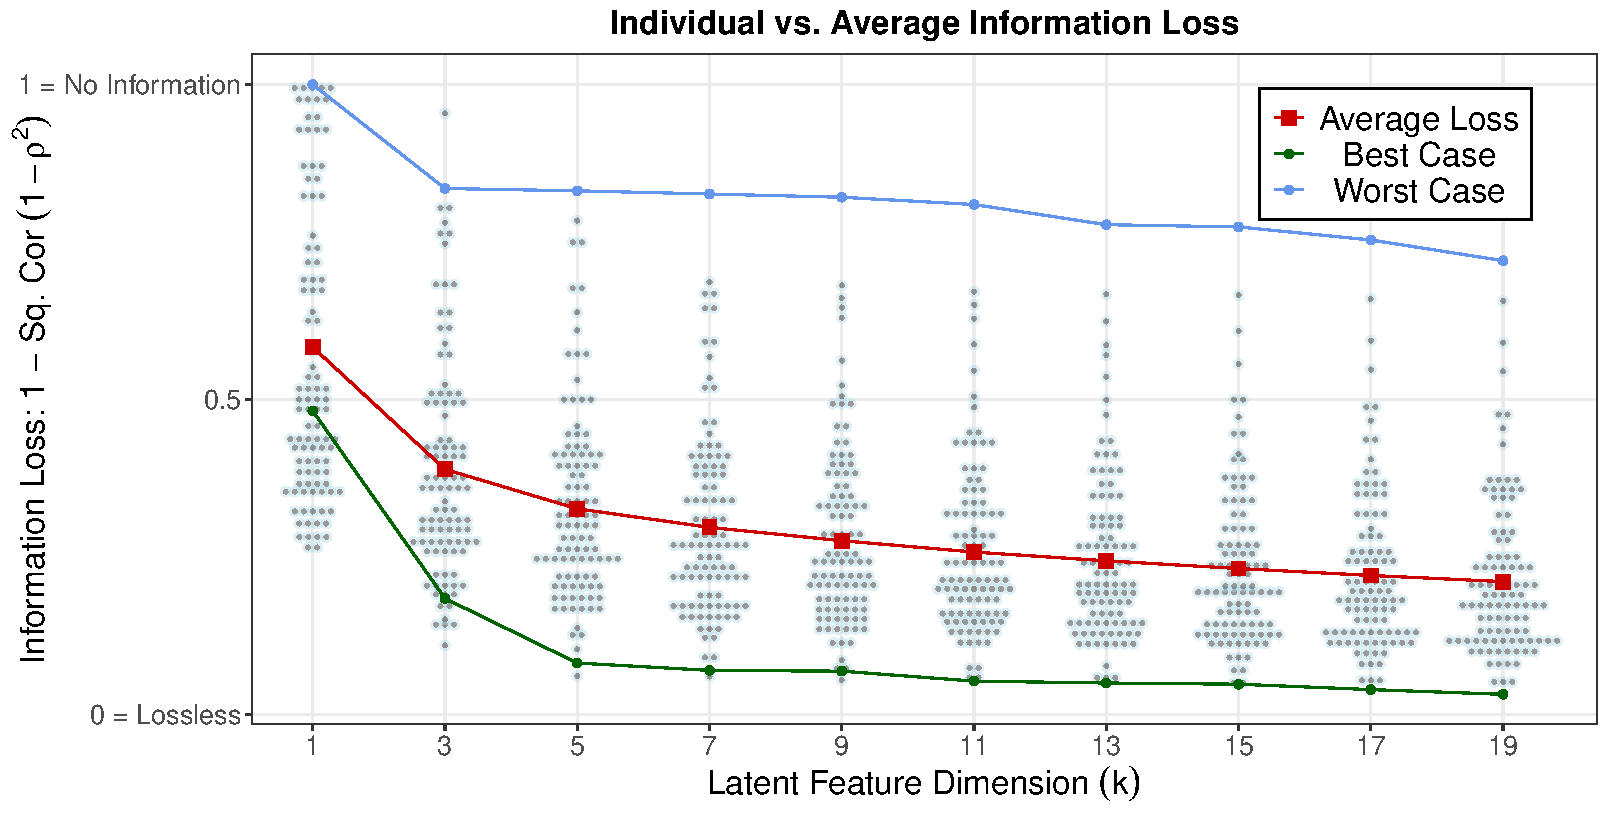
\includegraphics[width=0.75\textwidth]{figures/info-loss.pdf}
    \caption{Generalisation errors from a PCA representation of the \texttt{phoneme} data \parencite{hastie_elements_2009}. The grey dots represent individual cross-validated reconstruction errors from PCA representations using different numbers of latent features ranging from $1$ to $19$ ($x$ axis). 
    The squared correlation is used as reconstruction loss, so $0$ indicates no information retained by the representation and $1$ indicates a lossless representation ($y$ axis).
    The square red points and solid red line trace the average reconstruction error. The green and blue points / lines trace the performance of the best and worst performing observations (selected at $K=19$), respectively.}
    \label{fig:ind-losses}
\end{figure}


Achieving a chosen tolerance level for every observation (i.e., requiring that even the worst case meets the near-losslessness threshold) can sometimes be unrealistic in practice.
Often, a small number of observations (e.g., such as the one traced by the blue points and line in Figure \ref{fig:ind-losses}) possess indiosyncratic features that cannot be captured by a representation that is otherwise sparse and near-lossless for the majority of the observations.
In this case, using the worst case is overly stringent and results in a latent feature representation that is higher-dimensional and more complex than required for the majority of observations.
Therefore, we generalise the ideas the notion of near lossslessness of the entire dataset, and require it for is met for \emph{quantiles} or \emph{percentiles} of the distribution of individual generalisation errors, where the worst case observation is the $100$th percentile. 
As before, we $\epsilon$ denotes the tolerance level of information loss that we want to achieve.
We now introduce the \emph{cut-off criterion}, which we denote by $\alpha$ as the proportion of observations that we want to achieve this tolerance level.
For example, a cut-off criterion of $\alpha = 0.95$ would indicate that we require $95\%$ of the observations in the dataset to achieve a loss smaller than the tolerance level $\epsilon$.
Finally, if we fix $\epsilon$ and $\alpha$ and choose a representation method (e.g., PCA), then we use the term \emph{qualifying criterion (qc)} to denote the smallest latent feature dimension $K$ for which the criterion is achieved.
When comparing between two methods, for a fixed $\epsilon$ and $\alpha$, we prefer the method with a smaller qualifying criterion.

\subsection{Cross-validated Estimation of Information Loss}

Because we can view information loss as a measure of prediction, it is susceptible to \emph{overfitting}.
If we evaluate the information loss of a latent feature representation method on the same data used to learn that representation, then our information loss estimates will tend to be overly optimistic.
Typically, the information loss estimate will tend to be smaller than the method's true \emph{generalisation error}, which we define as its information loss in reconstructing unseen data.
To obtain a valid estimate of generalisation error, it is necessary to use an independent \emph{validation} dataset that is not used to learn the latent feature representation.
For example, Figure \ref{fig:training-validation} displays the average information loss in applying PCA to the Proteomic Gels data \parencite{morris_pinnacle_2008} on training and validation sets.
The training set estimate of information loss is overly optimistic and is much lower than the validation estimate.


Generally, with limited data, it is inefficient to perform a single split of the dataset into training and validation sets, as a single random split will tend to be variable (i.e., if the split were performed again, the new validation set would produce a different estimate of information loss) \parencite{harrell_jr_regression_2015}.
Additionally, because we are interested in the individual values of information loss (rather than an average), sample splitting would only provide us with these values for observations included in the validation set. 
To mitigate these concerns, we employ \emph{cross-validation} \parencite{stone_cross-validatory_1974}, where the data are systematically divided into different training and validation splits, called folds, and the training and validation is performed separately for each split.
When we are interested in an average or total estimate of information loss, cross-validation will tend to be more stable than sample splitting because the estimates are averaged over different folds.
For our purposes, it additionally produces a generlisation error estimate for each individual observation in the data.
Cross-validation has long been understood as a way to estimate generalisation error for latent feature representation methods, in particular PCA (e.g., dating back to the work of \textcite{wold_cross-validatory_1978, eastment_cross-validatory_1982}). 
However, it is not returned by default by standard software packages and is not routinely used to choose between different methods.

\begin{figure}
    \centering
    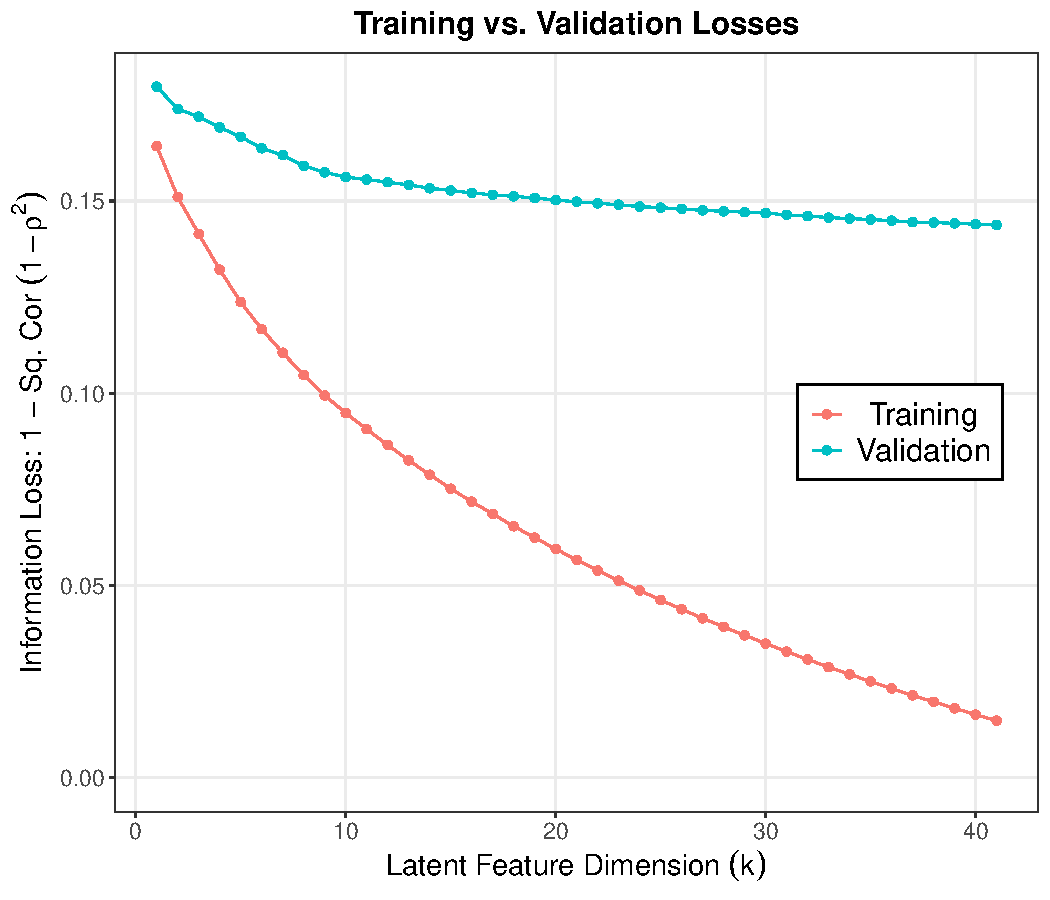
\includegraphics[width=0.5\linewidth]{figures/training-validation.pdf}
    \caption{Example of the average information loss from PCA of the Proteomic Gels data \parencite{morris_pinnacle_2008}, where the loss estimate is computed on the training sample (blue) vs. on a validation sample (red) (i.e., estimated via $5$-fold cross-validation).}
    \label{fig:training-validation}
\end{figure}

